\subsection{IMU 軸とジャイロ積分}

車輪エンコーダだけで差動二輪ロボットの姿勢を積分すると、左右輪の移動量差からヨー角を計算できる。しかし、片輪が短い時間だけ空転したり、床面で横滑りしたりすると、エンコーダは「車輪が進んだ量」を正しく数えても、「機体が床に対して向きを変えた量」を正しく表さない。オドメトリの式そのものは滑らかな軌跡を出すため、推定された向きのずれはすぐには見えにくい。数 m 走った後に、地図上の経路だけが少しずつ回転しているように見えることがある。この制限を補うため、車輪ではなく機体に固定された座標軸で角速度を測る IMU を導入する。

ここで必要なのは IMU の分類表ではなく、機体に貼り付いた測定軸である。床に固定された慣性系を $\{I\}$ とし、ロボットの中心に固定された機体系を $\{B\}$ とする。平面走行では、$\{B\}$ の $x_B$ 軸を前方、$y_B$ 軸を左方向、$z_B$ 軸を上向きに取る。慣性系の $x_I$ 軸から機体系の $x_B$ 軸まで反時計回りに測った角をヨー角 $\psi$ [rad] とする。ロボットが床から浮かず、ロールとピッチが小さい範囲では、$z_B$ 軸まわりの角速度 $\omega_z^B$ [rad/s] はヨー角の時間微分
\begin{equation}
  \dot{\psi}(t)=\omega_z^B(t)
\end{equation}
として扱える。この近似は、二輪ロボットの進行方向と横方向を機体に結び付け、地図上の向きだけを一つの角度で追うための平面モデルである。

ジャイロは角速度そのものを返すのではなく、バイアスとノイズを含む測定値を返す。時刻 $t_k=kT_s$、サンプリング周期 $T_s$ [s] の離散測定を
\begin{equation}
  \omega_{z,m,k}^B
  =
  \omega_z^B(t_k)+b_g+n_{g,k}
\end{equation}
と書く。$\omega_{z,m,k}^B$ は測定された $z_B$ 軸まわり角速度 [rad/s]、$b_g$ は一定とみなしたジャイロバイアス [rad/s]、$n_{g,k}$ は平均 0 の測定ノイズ [rad/s] である。角速度を時間で積分すると角度になるので、単位は
\begin{equation}
  [\mathrm{rad/s}]\,[\mathrm{s}]=[\mathrm{rad}]
\end{equation}
とそろう。

連続時間では、初期時刻 $t_0$ から時刻 $t$ までのヨー角は
\begin{equation}
  \psi(t)
  =
  \psi(t_0)+\int_{t_0}^{t}\omega_z^B(\tau)\,\dd\tau
\end{equation}
である。サンプリングされた測定値を 1 サンプルの間だけ一定とみなすと、ジャイロ積分は
\begin{equation}
  \hat{\psi}_k
  =
  \hat{\psi}_{k-1}
  +
  \left(\omega_{z,m,k}^B-\hat{b}_g\right)T_s
\end{equation}
となる。$\hat{b}_g$ はバイアスの補正値である。右辺の括弧の中は [rad/s]、$T_s$ は [s] なので、1 ステップで加える量は [rad] である。エンコーダのスリップで壊れた「車輪から見た向き」ではなく、機体に固定されたジャイロの角速度を積分して向きを進める点が、IMU を入れる最初の利点である。

ただし、ジャイロ積分は絶対的な方位を直接測っているわけではない。真の角度を同じサンプリングで
\begin{equation}
  \psi_k
  \simeq
  \psi_{k-1}+\omega_z^B(t_k)T_s
\end{equation}
と近似し、誤差を $e_{\psi,k}=\hat{\psi}_k-\psi_k$ と置く。測定式と積分式を代入して差を取ると
\begin{align}
  e_{\psi,k}
  &=
  e_{\psi,k-1}
  +
  \left(b_g-\hat{b}_g+n_{g,k}\right)T_s
\end{align}
である。バイアスを補正しない場合は $\hat{b}_g=0$ であり、$E[n_{g,k}]=0$、$e_{\psi,0}=0$ とすれば
\begin{align}
  E[e_{\psi,k}]
  &=
  E[e_{\psi,k-1}]+b_gT_s\\
  &=
  kb_gT_s\\
  &=
  b_g t_k
\end{align}
となる。一定のバイアスは 1 サンプルごとには小さくても、時間に比例する角度誤差として蓄積する。

図\ref{fig:flow-six-imu-gyro-examples}は、機体系に固定された IMU の軸と、一定バイアスを補正しないときのヨー角誤差を並べたものである。右図では $T_s=0.01\,\mathrm{s}$ とし、$b_g=0.1^\circ/\mathrm{s}$、$0.5^\circ/\mathrm{s}$、$1.5^\circ/\mathrm{s}$ の三つを比較している。$0.5^\circ/\mathrm{s}$ は 100 Hz の 1 サンプルでは $0.005^\circ$ しか増えないが、60 s 後には
\begin{equation}
  0.5^\circ/\mathrm{s}\times 60\,\mathrm{s}=30^\circ
\end{equation}
の向き誤差になる。$1.5^\circ/\mathrm{s}$ なら同じ 60 s で $90^\circ$ まで増える。小さな直流成分が積分で大きな低周波誤差になるため、ジャイロはスリップに強い一方で、バイアスを無視したまま長時間の方位基準として使うことはできない。

\begin{figure}[tb]
\centering
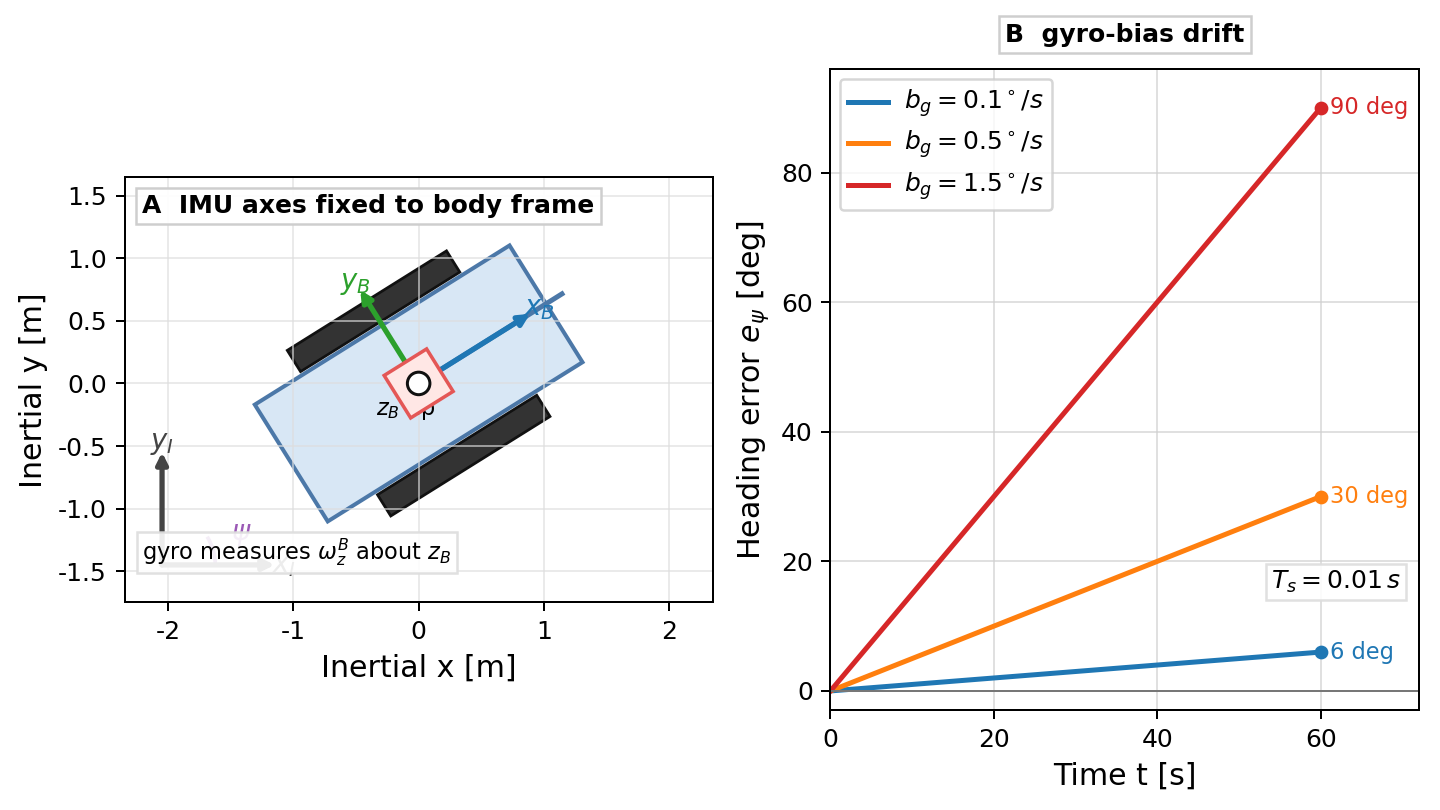
\includegraphics[width=0.95\linewidth,bb=0 0 1440 810]{figures/flow6_imu_gyro_examples.png}
\caption{差動二輪ロボットに固定した IMU の機体軸と、一定ジャイロバイアスによるヨー角誤差の蓄積。左図では IMU が機体系 $\{B\}$ に固定され、$z_B$ 軸まわりの角速度を測る。右図では $T_s=0.01\,\mathrm{s}$ でジャイロを積分し、バイアスが $0.1^\circ/\mathrm{s}$、$0.5^\circ/\mathrm{s}$、$1.5^\circ/\mathrm{s}$ のとき、誤差がそれぞれ 60 s 後に $6^\circ$、$30^\circ$、$90^\circ$ へ達することを示している。}
\label{fig:flow-six-imu-gyro-examples}
\end{figure}

この比較から、IMU を入れる意味は二つに分かれる。第一に、車輪が滑った瞬間でも、機体が実際に回った角速度を直接測れるので、エンコーダだけの向き推定よりスリップに引きずられにくい。第二に、ジャイロだけではバイアスが積分されるため、長時間の向きには別の情報が必要になる。加速度計が測る比力と重力方向からロール・ピッチを扱う話はこの後の段階で扱うが、ここではまだその導出には進まない。まず押さえるべき事実は、IMU の軸は機体に固定されており、ジャイロ測定は角速度として有用だが、積分するとバイアスが角度誤差へ変わるという点である。
